\documentclass[slidestop,compress,mathserif]{beamer}

\usepackage[portuges]{babel}
\usepackage[utf8]{inputenc}
\usepackage{epsfig}
\usepackage{graphicx}
%\usepackage{indentfirst}
\usepackage{fancyhdr}
\usepackage{algorithm-br}
\usepackage{algorithmic-br}

%\usepackage{hyperref}
%\usepackage{colortbl}
\usepackage{amssymb}

%\usepackage[font=small,format=plain,labelfont=bf,up,textfont=it,up]{caption}

%\usetheme{Berlin}
\usetheme{Antibes}
\usecolortheme{lily}

\setbeamercovered{transparent}

\title{\emph{Um Algortimo Genético para a o Problema da Mochila Compartimentada} }
\author{Pedro Henrique Neves da Silva}
\date{\today}

%inicio da seção principal do documento
\begin{document}

%inicio de um novo slide
\begin{frame}
\titlepage
\end{frame}


\section{Introducão}
\begin{frame} {Introdução}

O Problema da Mochila
\begin{itemize}
\item Desperta muito interesse devido a sua vasta gama de aplicações
\item Surge como subproblema de inúmeros outros problemas 
\item  Possui diversas variantes agrupadas no que podem ser chamadas de Classes de Problemas da Mochila
\item Se caracteriza, basicamente, pela escolha de um subconjunto de itens que irá otimizar um objetivo
\item Cada item deve possuir um ``peso'' e um ``benefício'' e a mochila deve possuir uma capacidade máxima
\item Deseja-se escolher um subconjunto de itens que maximize o benefício da mochila, sem que a soma dos pesos dos itens selecionados ultrapasse a capacidade da mochila

\end{itemize}
\end{frame}


\section{Problema da Mochila}

\subsection{Classes de Problemas da Mochila}
\begin{frame} {Problema da Mochila} {Classes de Problemas da Mochila}


\begin{itemize}
 \item Todas as mochilas que serão apresentados nessa seção utilizam um conjunto de itens $S$ com $n$ itens, cada item $i$ ($1 \leq i \leq n$) deve estar associado a um valor de benefício $b_i$ e um peso $l_i$. A capacidade da mochila é representada por $L$.

\end{itemize}

\end{frame}


\begin{frame} {Problema da Mochila} {Problema da Mochila 0-1}

\begin{itemize}
\item Para cada item $i \in S$ é associada a variável $x_i$ que pode assumir um dos dois valores: 0 ou 1. $x_i$ será 0 quando o item $i$ não for escolhido para compor a mochila, e será 1 quando o item fizer parte da solução.
\end{itemize}

\begin{eqnarray}
	Maximizar & \displaystyle \sum_{i = 1}^{n} b_ix_i \\
	Sujeito \ a & \displaystyle \sum_{i = 1}^{n} l_ix_i \leq L \\
	& x_i = 0 \ ou \ 1, \ i = 1, ..., n \nonumber
\end{eqnarray}
\end{frame}

%\begin{frame} {Problema da Mochila} {Problema da Mochila Fracionária} 

%\scriptsize
%Se não houver a restrição de \textit{aceitar} ou \textit{recusar} um item de $S$ para fazer parte da solução, e tivermos a possibilidade  de escolher uma porção do item para fazer parte da solução, teremos a versão fracionária do Problema da Mochila. Deseja-se, então, encontrar a porção $x_i$ do item $i$ que fará parte da solução, tal que:

%\begin{eqnarray}
%	Maximizar & \displaystyle \sum_{i \in S} b_i(x_i/l_i) \\
	%Sujeito \ a & \displaystyle \sum_{i = 1}^{n} l_ix_i \leq L \\
	%& 0 \leq x_i \leq l_i \ para \ cada \ i \in S \nonumber
%\end{eqnarray}

%\end{frame}


\begin{frame} {Problema da Mochila} {Problema da Mochila Restrita}

\begin{itemize}
 \item Variáveis deixam de ser binárias e passam a indicar o número de repetições do respectivo item na mochila
 \item Cada variável tem associada a ela um limitante inferior ($t_i$) e um superior ($d_i$)
\end{itemize}

\begin{eqnarray}
	Maximizar & \displaystyle \sum_{i=1}^n b_i x_i \\
	Sujeito \ a & \displaystyle \sum_{i=1}^n l_i x_i  \leq L \\
	&  t_i \leq x_i \leq d_i \ e \ inteiro, i=1,...,n  \nonumber
\end{eqnarray}

\end{frame}


%\begin{frame} {Problema da Mochila} {Problema da Soma de Subconjuntos}

%Esse tipo de mochila se aproxima muito da classe de mochilas com variáveis binárias. A diferença se restringe à função objetivo onde o benefício é substituído pelo peso do item. Esta nova abortagem é útil quando é necessário selecionar um subconjunto de itens, cuja soma de seus pesos se aproxime ao máximo, mas não exceda, a capacidade da mochila. Segue o modelo matemático equivalente:

%\begin{eqnarray}
%	Maximizar & \displaystyle \sum_{i=1}^n l_i x_i \\
%	Sujeito \ a & \displaystyle \sum_{i=1}^n l_i x_i  \leq L \\
%	& x_i=0 \ ou \ 1, i=1,...,n \nonumber
%\end{eqnarray}

%\end{frame}


\begin{frame} {Problema da Mochila} {Problema de Múltiplas Mochilas 0-1}

\scriptsize
\begin{itemize}
 \item $n$ conjuntos de itens, disjuntos entre si
 \item Conjunto com $m$ mochilas, cada uma com capacidade $L_j$, $(1 \leq j \leq m)$
 \item Itens de um determinado conjunto podem ser atribuídos a, no máximo, uma única mochila 
 
\end{itemize}

\begin{eqnarray}
	Maximizar & \displaystyle \sum_{j=1}^m \sum_{i=1}^n b_i x_{ij} \\
	Sujeito \ a & \displaystyle \sum_{i=1}^n l_i x_{ij} \leq L_j, j=1,...,m \\
	& \displaystyle \sum_{j=1}^m x_{ij} \leq 1, i=1,...,n \\
	& x_{ij}=0 \ ou \ 1, i=1,...,n , j=1,...,m \nonumber
\end{eqnarray} 

\end{frame}


\subsection{Estratégias para Resolução de Mochilas}
\begin{frame} {Problema da Mochila} {Estratégias para Resolução de Mochilas}

\begin{itemize}
\item Embora o Problema da Mochila 0-1 e suas variações sejam pertencentes à classe NP-difícil, muitos deles surgem em aplicações práticas na vida real ou como sub-problemas de outros problemas mais complexos e por isso justifica-se a tentativa de encontrar soluções exatas ou aproximadas, mesmo que isso custe muito tempo.
\end{itemize}

\end{frame}


\begin{frame} {Problema da Mochila} {Branch-and-Bound}

\begin{itemize}
\item Funciona como o método de força bruta, porém, utiliza um mecanismo para diminuir o conjunto de configurações, descartando a verificação daquelas que não tenham chance de serem soluções ótimas.

\item Para descartar configurações não promissoras, calcula-se um \textit{limitante} que é o valor máximo (ou mínimo) que uma solução pode atingir a partir da configuração em questão. Se esse valor limitante não for satisfatório, essa configuração será descartada.
\end{itemize}
\end{frame}


%\begin{frame} {Problema da Mochila} {Branch-and-Bound}

%\begin{itemize}
%\item  Utilizaremos um limite superior para o seu valor potencial: dada uma configuração $c$ que considera os itens de índice $0$ a $i$, calculamos um limite superior para $c$ iniciando com o valor total $l_c$ de $c$ e verificando quanto valor a mais podemos colocar em $c$ se aumentarmos $c$ com uma solução para o problema fracionário da mochila que seja retirada dos itens restantes em $S$.


%\end{itemize}

%\end{frame}

\begin{frame} {Problema da Mochila} {Branch-and-Bound}

\begin{itemize}
\item Seja $s_c$ o somatório dos pesos de todos os itens que compõem a configuração $c$
\item Seja $k$ o maior valor tal que $\sum_{j=i+1}^{k} s_j \leq L-s_c$
\item Os itens de $i+1$ a $k$ são os melhores itens que ainda cabem na mochila 
\item Para calcular o limite superior para $c$, consideramos a adição de todos esses elementos a $c$ mais tudo o que for possível do item $k+1$ 

\begin{equation}
 upper(c)= l_c+ \sum_{j=i+1}^{k} l_j + (L-s_c-\sum_{j=i+1}^{k} s_j) (l_{k+1})/(s_{k+1})
\end{equation} 


\end{itemize}

\end{frame}



\begin{frame} {Problema da Mochila} {Programação Dinâmica}

\begin{itemize}
\item Os itens de $S$ serão numerados como 1,2,3,...,$n$
\item Para cada $k \in \{1,2,...,n\}$, define-se $S_k$ como o subconjunto contendo itens $S$ rotulados de 1 até $k$
\item Teremos $B[0,w]=0$ para cada $w \leq L$ e derivaremos a seguinte relação para o caso geral:

\[ B[k,w]= \left \{ \begin{tabular}  {lc}
                                     $B[k-1,w]$ & $:l_k > w$ \\
                                     $max\{ B[k-1,w], B[k-1,w-l_k]+b_k\}$ & $:l_k \leq w$ \\
                                  \end{tabular} \right. \]
\end{itemize}
\end{frame}


\begin{frame} {Problema da Mochila} {Algoritmo Genético}

\begin{itemize}
 \item Os algoritmos genéticos são uma família de modelos computacionais inspirados na evolução
 \item Algoritmos genéticos não garantem que a melhor solução será encontrada
 \item Indicados para encontrar soluções aproximadas para problemas de otimização difíceis que envolvem um grande número de variáveis
 \item Trabalham com descrições de entrada formadas por cadeias de bits de tamanho fixo
 \item Começa com uma população aleatória de cromossomos
 \item Essas estruturas são avaliadas e associadas a uma probabilidade de reprodução
\end{itemize}

\end{frame}

\begin{frame} {Problema da Mochila} {Algoritmo Genético}

\begin{description}
	\item[gene] um ou mais símbolos do alfabeto
	\item[cromossomo] conjunto de genes que corresponde a um indivíduo
	\item[população] conjunto de indivíduos que corresponde ao conjunto de pontos no espaço de busca 
	\item[geração] iteração completa do algoritmo genético que gera uma nova população 
	\item[aptidão] saída gerada pela função objetivo para um indivíduo da população.
\end{description}

\end{frame}


\begin{frame} {Problema da Mochila} {Fluxograma do Algoritmo Genético}

\begin{figure}[htp]
	\centering
	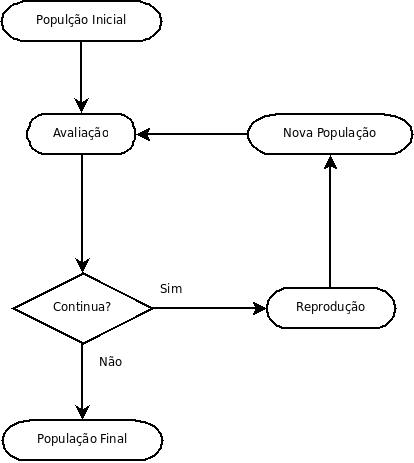
\includegraphics[scale=0.4]{images/fluxo.jpg}
	%\caption{\tiny{Fluxograma do algoritmo genético.}}
	\label{fig:fluxo}
\end{figure}

\end{frame}


\begin{frame} {Problema da Mochila} {Algoritmo Genético}

\begin{description}

	\item[Cálculo de Aptidão] determinada por meio do cálculo da função objetivo

	\item[Fase de Seleção] os indivíduos mais aptos da geração atual são selecionados.

	\item[Fase de Cruzamento] um novo cromossomo é gerado permutando-se a partes de um cromossomo com partes do outro.

	\item[Fase de Mutação] utilizada para garantir uma maior varredura do espaço de busca.

	\item[Outros parâmetros] existem vários parâmetros que podem melhorar o seu desempenho.

\end{description}

\end{frame}


\begin{frame} {Problema da Mochila} {Algoritmo Genético}

\begin{figure}[htp]
	\centering
	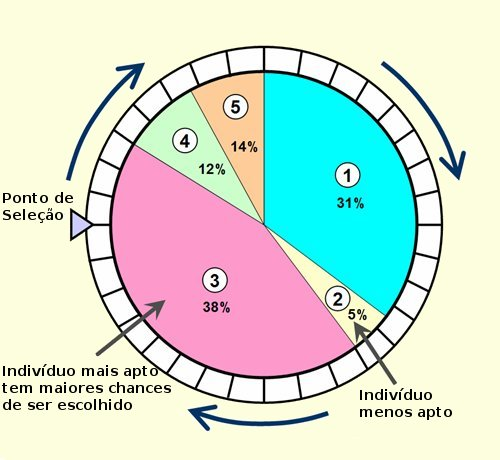
\includegraphics[scale=0.3]{images/roleta.jpg}
	\caption{Exemplo de seleção por roleta.}
	\label{fig:roleta}
\end{figure}

\end{frame}


\section{Problema da Mochila Compartimentada}
\subsection{Definição}
\begin{frame} {Problema da Mochila Compartimentada} {Definição}

\begin{itemize}
 \item É uma variação do Problema da Mochila
 \item Itens estão divididos em classes
 \item Mochila pode ser dividida em compartimentos com capacidades flexíveis 
\item Consiste em determinar a melhor distribuição dos itens em compartimentos, visando maximizar o benefício total, levando em consideração as capacidades máximas e mínimas de cada compartimento e a capacidade máxima da mochila
\end{itemize}

\end{frame}


\begin{frame} {Problema da Mochila Compartimentada} {Definição}

\begin{description}
	\item[$M=\{1,...,m\}$] conjunto dos tipos de itens;
	\item[$K$] quantidade de classes distintas (ou partições);
	\item[$C_k$] subconjunto de $M$, contendo itens de mesma classe, $k=1,...,K$ (para $i \neq j$, $C_i  \bigcap C_j = \emptyset$);
	\item[$c_k$] custo de incluir um compartimento para itens da classe $k$ na mochila ($c_{k} \geq 0$), $k = 1, ..., K$;
	\item[$S$] perda decorrente da inclusão de um novo compartimento na mochila;
	\item[$L$] capacidade da mochila;
	\item[$N_k$] número total de possíveis compartimentos para a classe $k$;
\end{description}

\end{frame}


\begin{frame} {Problema da Mochila Compartimentada} {Definição}

\begin{description}
	\item[$L_{max}$] capacidade máxima de cada compartimento;
	\item[$L_{min}$] capacidade mínima de cada compartimento ($L_{min} < L_{max} < L$);
	\item[$l_i$] peso do item $i$ ($l_i >0$), $i = 1, ..., m$; 
	\item[$b_i$] benefício ou utilidade do item $i$ ($b_i \geq 0$), $i=1,...,m$;
	\item[$d_i$] limite máximo de itens $i$ na mochila, $i = 1, ..., m$;
	\item[$\alpha_{ijk}$] número de itens do tipo $i$, da classe $k$, no compartimento do tipo $j$ ($i = 1, ..., m, k = 1, ..., K$ e $j = 1, ..., N_{k}$); e
	\item[$\beta_{jk}$] número de repetições do compartimento do tipo $j$ alocados com a classe $k, k = 1, ..., K$ e $j = 1, ..., N_{k}$.
\end{description}

\end{frame}


\begin{frame} {Problema da Mochila Compartimentada} {Definição}

\begin{itemize}
	\item Capacidade ocupada dada por:
	\begin{eqnarray}
		L_{jk}: \sum_{i \in C_{k}}l_{i}\alpha_{ijk}, & k = 1, ..., K \ e \ j = 1, ..., N_{k}.
	\end{eqnarray}

	\item Valor de utilidade, ou benefício, dado por:
	\begin{eqnarray}
		V_{jk}: \sum_{i \in C_{k}}b_{i}\alpha_{ijk}, & k = 1, ..., K \ e \ j = 1, ..., N_{k}.
	\end{eqnarray}

\end{itemize} 

\end{frame}

\begin{frame} {Problema da Mochila Compartimentada} {Definição}


\begin{eqnarray}
	Maximizar: & \displaystyle \sum_{k = 1}^{K}\sum_{j = 1}^{N_{k}}(V_{jk} - c_{l})\beta_{jk} \\
	Sujeito \ a: &  \displaystyle V_{jk} = \sum_{i \in C_{k}}b_{i}\alpha_{ijk}\\
	& \displaystyle L_{jk} = \sum_{i \in C_{k}}l_{i}\alpha_{ijk} \\
	& \displaystyle L_{min} \leq L_{jk} \leq L_{max} 
\end{eqnarray}

\end{frame}


\begin{frame} {Problema da Mochila Compartimentada} {Definição}

\begin{eqnarray}
	& \displaystyle \sum_{k = 1}^{K}\sum_{j = 1}^{N_{k}}\alpha_{ijk}\beta_{jk} \leq d_{i}, i = 1, ..., m \\
	& \displaystyle \sum_{k = 1}^{K}\sum_{j = 1}^{N_{k}}(L_{jk} + S)\beta_{jk} \leq L \\
	& \displaystyle \alpha_{ijk} \geq 0, \ inteiro \ e \nonumber\\
	& \displaystyle \beta_{jk} \geq 0, \ inteiro, \nonumber\\
	& \displaystyle para \ i = 1, ..., m, \ k = 1, ..., K \ e \ j = 1, ..., N_{k}. \nonumber
\end{eqnarray}

\end{frame}


\subsection{Simplificações Adotadas}
\begin{frame} {Problema da Mochila Compartimentada} {Simplificações adotadas}

\begin{itemize}
 \item As simplificações adotadas não alteram a natureza do problema nem a sua complexidade computacional
\end{itemize}

\begin{itemize}
	\item $N_K=1$, ou seja, existe apenas 1 compartimento para a classe $k$;
	\item $L_{min}=0$, ou seja, uma classe $k$ de itens pode estar presente, ou não, em algum compartimento na mochila; e
	\item $0 \leq d_i \leq 1$, ou seja, cada item pode aparecer no máximo 1 vez na solução.
\end{itemize}

\end{frame}


\begin{frame} {Problema da Mochila Compartimentada} {Simplificações adotadas}

\begin{eqnarray}
	Maximizar: & \displaystyle \sum_{k = 1}^{K}(V_{jk} - c_{l}) \\
	Sujeito \ a: &  \displaystyle V_{k} = \sum_{i \in C_{k}}b_{i}\alpha_{ik} \\
	& \displaystyle L_{k} = \sum_{i \in C_{k}}l_{i}\alpha_{ik} \\
	& \displaystyle 0 \leq L_{jk} \leq L_{max} \\
	& \displaystyle \sum_{k = 1}^{K}(L_{k} + S) \leq L \\
	& \displaystyle \alpha_{ik} \geq 0, \ inteiro \ e \nonumber\\
	& \displaystyle para \ i = 1, ..., m \ e \ k = 1, ..., K \nonumber
\end{eqnarray}

\end{frame}


\subsection{Técnicas de Implementação}
\begin{frame} {Problema da Mochila Compartimentada}

\begin{itemize}
 \item Existem várias heurísticas para se resolver o Problema da Mochila Compartimentada
 \item Destacarei a heurística da decomposição e o uma possível implementação de um algoritmo genético para a mochila compartimentada do caso restrito. 
\end{itemize}

\end{frame}


\begin{frame} {Problema da Mochila Compartimentada} {Heurística da Decomposição}

\begin{itemize}
 \item Consiste de duas fases:
\begin{itemize}
\item Na primeira, são resolvidos $(K-1)$ Problemas da Mochila de capacidade $L_{max}$, um para cada agrupamento
\item Na segunda fase, um problema clássico da mochila é resolvido
\end{itemize}
\end{itemize}

\begin{eqnarray}
	Maximizar: & \displaystyle V_{k} = \sum_{i \in C_{k}}p_{i}\alpha_{ik} \\
	Sujeito \ a: & \displaystyle \sum_{i \in C_{k}}l_{i}\alpha_{ik} + S \leq L_{max} \\
	& \displaystyle 0 \leq \alpha_{ik} \leq d_{i} \ e \ inteiro, \ i = 1, ..., m. \nonumber
\end{eqnarray}

\end{frame}


\begin{frame} {Problema da Mochila Compartimentada} {Heurística da Decomposição}

\begin{eqnarray}
	Maximizar: & \displaystyle \sum_{k = 1}^{K}(V_{k} - c_{k})\beta_{k} \\
	Sujeito \ a: & \displaystyle \sum_{k = 1}^{K}L_{k}\beta_{k} \leq L - S \\
	& \displaystyle \alpha_{ik}\beta_{k} \leq d_{i}, \ i \in C_{k} \ e \ k = 1, ..., K \nonumber \\
	& \beta_{k} \geq 0, \ inteiro \ para \ k  = 1, ..., K. \nonumber
\end{eqnarray}

\end{frame}


\begin{frame} {Problema da Mochila Compartimentada} {Algoritmo Genético}

\begin{itemize}
 
 \item Funciona como a heurística de decomposição
 \item Em cada indivíduo são computados os pesos e é verificado se, para cada compartimento, o valor obtido é menor que o limite do compartimento, depois é verificado se o peso total ultrapassa o limite da mochila
 \item Duas aptidões: uma para o peso e outra para o benefício
 \item Denominaremos de {\it razão de aproximação} a divisão do valor da solução ótima pelo valor retornado pelo algoritmo genético
 \item Quanto mais próximo de 1, mais próximo do valor ótimo será a resposta do algoritmo genético
\end{itemize}

\end{frame}


\begin{frame} {Implementações e Resultados Computacionais} {Problema da Mochila 0-1}


\begin{itemize}

\item Força-bruta, programação dinâmica, branch-and-bound e algoritmo genético
\item Parâmetros utilizados no algoritmo genético:

\begin{itemize}
	\item Número de gerações: 50.
	\item Tamanho da população: 30.
	\item Taxa de \textit{cross-over}: 75\%.
	\item Taxa de mutação: 5\%.
\end{itemize}

\end{itemize}
\end{frame}


\begin{frame} {Implementações e Resultados Computacionais} {Problema da Mochila 0-1}

\scriptsize
\begin{figure}[htp]
	\centering
	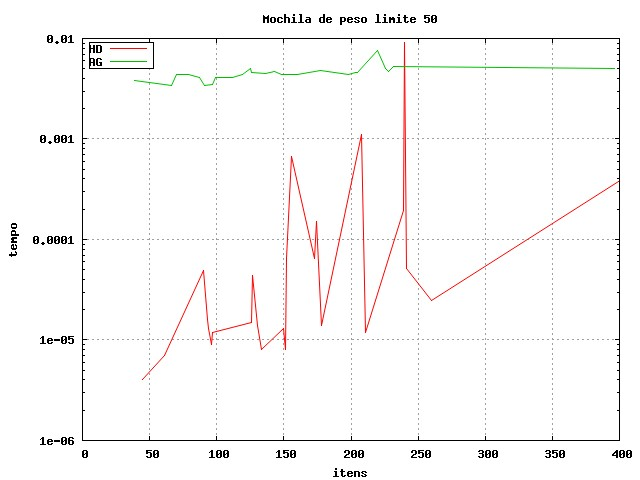
\includegraphics[scale=0.3]{images/w50.jpg}
	\caption{\tiny{Gráfico comparativo dos tempos de execução dos quatro métodos: força bruta(FB), branch-and-bound(BB), programação dinâmica(PD) e algoritmos genéticos(AG), para mochilas com capacidade 50.}}
\end{figure}

\end{frame}


\begin{frame} {Implementações e Resultados Computacionais} {Problema da Mochila 0-1}

\scriptsize
\begin{figure}[htp]
	\centering
	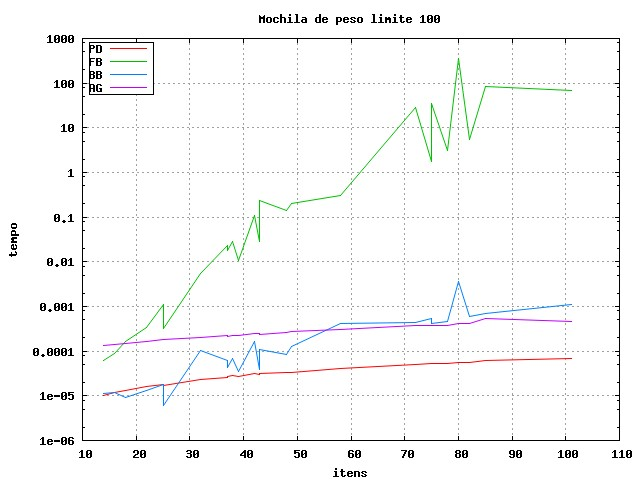
\includegraphics[scale=0.3]{images/w100.jpg}
	\caption{\tiny{Gráfico comparativo dos tempos de execução dos quatro métodos: força bruta(FB), branch-and-bound(BB), programação dinâmica(PD) e algoritmos genéticos(AG), para mochilas com capacidade 100.}}
\end{figure}

\end{frame}


\begin{frame} {Implementações e Resultados Computacionais} {Problema da Mochila 0-1}

\scriptsize
\begin{figure}[htp]
	\centering
	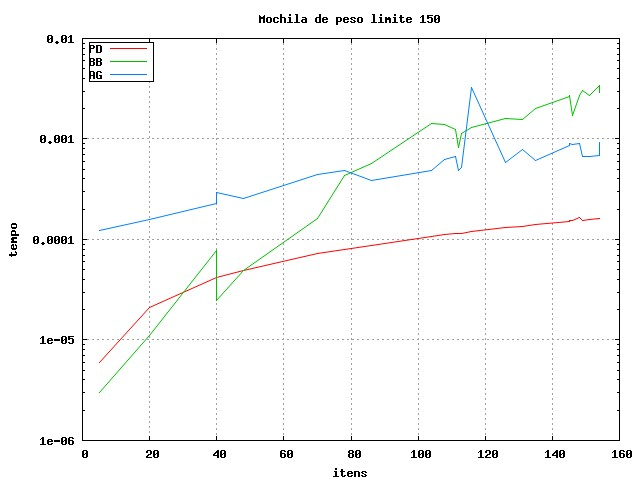
\includegraphics[scale=0.3]{images/w150.jpg}
	\caption{\tiny{Gráfico comparativo dos tempos de execução dos três métodos mais rápidos: branch-and-bound(BB), programação dinâmica(PD) e algoritmos genéticos(AG), para mochilas com capacidade 150.}}
\end{figure}

\end{frame}


\begin{frame} {Implementações e Resultados Computacionais} {Problema da Mochila 0-1}

\scriptsize
\begin{figure}[htp]
	\centering
	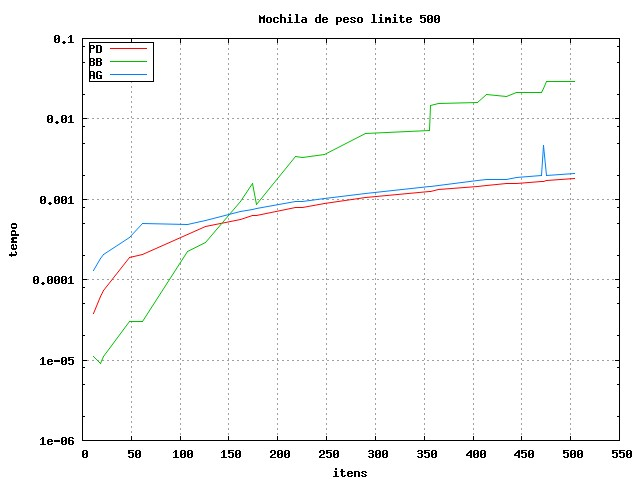
\includegraphics[scale=0.3]{images/w500.jpg}
	\caption{\tiny{Gráfico comparativo dos tempos de execução dos três métodos mais rápidos: branch-and-bound(BB), programação dinâmica(PD) e algoritmos genéticos(AG), para mochilas com capacidade 500.}}
\end{figure}

\end{frame}


\begin{frame} {Implementações e Resultados Computacionais} {Problema da Mochila 0-1}

\scriptsize
\begin{figure}[htp]
	\centering
	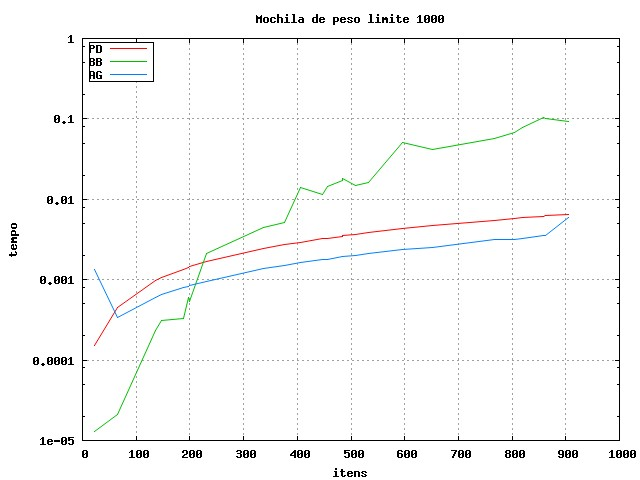
\includegraphics[scale=0.3]{images/w1000.jpg}
	\caption{\tiny{Gráfico comparativo dos tempos de execução dos três métodos mais rápidos: branch-and-bound(BB), programação dinâmica(PD) e algoritmos genéticos(AG), para mochilas com capacidade 1000.}}
\end{figure}

\end{frame}


\subsection{Problema da Mochila Compartimentada}
\begin{frame} {Implementações e Resultados Computacionais} {Problema da Mochila Compartimentada}

\begin{itemize} 
 \item Heurística de Decomposição:
\begin{itemize}
 \item Utiliz $K - 1$ chamadas ao algoritmo que utiliza força bruta para que escolher os melhores compartimentos
 \item Faz uma última chamada ao mesmo algoritmo, para que sejam escolhidos os compartimentos que entraram na mochila
\end{itemize}
\item Algoritmo Genético, com parâmatros: 

\begin{itemize}
	\item Número de gerações: 50.
	\item Tamanho da população: 30.
	\item Taxa de \textit{cross-over}: 75\%.
	\item Taxa de mutação: 5\%.
\end{itemize}

\end{itemize}


\end{frame}


\begin{frame} {Implementações e Resultados Computacionais} {Problema da Mochila Compartimentada}

\scriptsize
\begin{figure}[htp]
	\centering
	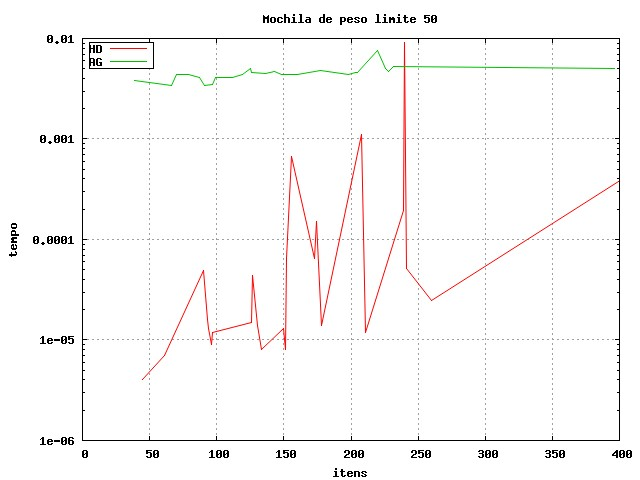
\includegraphics[scale=0.3]{images/com_w50.jpg}
	\caption{\tiny{Gráfico comparativo dos tempos de execução dos dois métodos: heurística da decomposição(HD) e algoritmos genéticos(AG), para mochilas com capacidade 50.}}
	\label{fig:com_w50}
\end{figure}

\end{frame}


\begin{frame} {Implementações e Resultados Computacionais} {Problema da Mochila Compartimentada}

\scriptsize
\begin{figure}[htp]
	\centering
	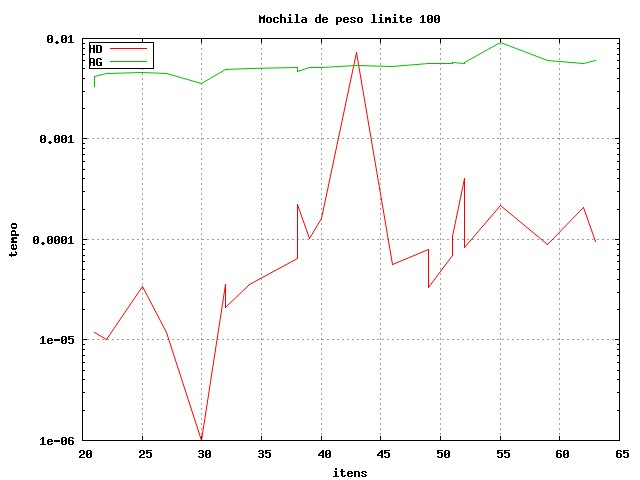
\includegraphics[scale=0.3]{images/com_w100.jpg}
	\caption{\tiny{Gráfico comparativo dos tempos de execução dos dois métodos: heurística da decomposição(HD) e algoritmos genéticos(AG), para mochilas com capacidade 100.}}
\end{figure}

\end{frame}


\section{Considerações Finais}
\begin{frame} {Conclusão}

\begin{itemize}
\item Para o Problema da Mochila 0-1, o algoritmo genético apresentou bons resultados
\item A razão de aproximação obtida foi igual a 1,13
\item Com relação ao Problema da Mochila Compartimentada, o algoritmo genético apresentou bom desempenho
\item Porém não há como avaliar com precisão quão próxima da solução ótima está a resposta do algoritmo
\item As soluções tem razão de aproximação próxima a 2.
\item Os algoritmos genéticos tem apresentado boas razões de aproximação, porém não podemos dizer que sejam algoritmos aproximativos
\end{itemize}

\end{frame}

\begin{frame}[allowframebreaks]{Referências}

\scriptsize
\nocite{*}
\bibliographystyle{alpha}
\bibliography{referencia}
\end{frame}


\end{document}
